\documentclass[11pt,a4paper]{article}
%\documentclass[10pt,twocolumn]{article}

\usepackage{Movements} %% cibler doc/modules/
\setlength{\columnsep}{1cm}


%\onecolumn
\begin{document}
  \fairetitre{Amélioration de la réactivité des réseaux pair à pair pour les MMOGs}{Étude bibliographique sur les déplacements en groupe dans les MMOG}{Xavier Joudiou}{Sergey Legtchenko \& Sébastien Monnet}{10/06/10}

\newpage
%\onecolumn
\tableofcontents
\newpage
%\twocolumn

\noindent{\textbf{Résumé}}\\
	\par \textit{Depuis plusieurs années, un nouveau type d'architecture des systèmes est apparu. Il s'agit de l'architecture pair à pair, cette architecture est devenue populaire grâce à des applications de partage de fichiers. Nous allons nous intéresser aux jeux vidéos massivement multijoueur (MMOG pour Massively Multiplayer Online Games) qui sont de plus en plus populaires et qui font ressortir des problèmes que l'architecture pair à pair doit pouvoir corriger. Le problème du passage à l'échelle sera l'un des plus importants à résoudre pour permettre à un grand nombre de joueurs de participer simultanément. Nous verrons comment l'architecture pair à pair peut être une des solutions.\\ 
	 Pour remédier à cela, une solution consiste à remplacer le modèle client/serveur par un réseau logique pair à pair (overlay). Malheureusement, les protocoles pair à pair existants sont trop peu réactifs pour assurer la faible latence nécessaire à ce genre d’applications. Néanmoins, quelques travaux ont déjà été menés pour adresser ce problème. L’idée est d’adapter le voisinage de chaque pair afin que toute l’information dont il aura besoin dans l'avenir se trouve proche de lui dans le réseau. Il est alors nécessaire de correctement évaluer les futurs besoins de chaque pair, et de faire évoluer son voisinage à temps. Dans ce rapport bibliographique, nous allons étudier les mouvements de groupe et ainsi nous pourrons voir si cette piste est exploitable pour l'amélioration de la réactivité des réseaux pair à pair pour les MMOG.}\\


\section{Introduction}
Dans ce document, nous allons étudier les déplacements en groupe des avatars dans les MMOG. Nous pourrons voir, grâce à cette étude rapide, si l'utilisation des déplacements en groupe est une piste intéressante dans l'amélioration du travail Blue Banana~\cite{191}. Le jeux en groupe (guilde et communauté) est un part importante de l'expérience que le joueur recherche en jouant à des MMOG~\cite{1501834,1255052}.

\newpage
\section{Les MMOG, des jeux socialisant?}
Sans rentrer dans des détails sur la vie sociale "réelle" des joueurs, nous allons étudier les comportements sociaux des joueurs. Ceci nous permettra de définir si un modèle de mobilité et des améliorations de la réactivité sont possibles.
\subsection{Différences en fonction du niveau du joueur}
Dans~\cite{1124834}, les auteurs se sont intéressés aux dynamiques sociales dans les MMOG, et particulièrement dans le jeu World Of Warcraft~\cite{wow}. Unes des premières observations et que les joueurs vont jouer différemment en fonction de leur niveau. Par exemple, les joueurs vont passés moins de temps au niveau 39, car à partir du niveau 40 les joueurs pourront se déplacer plus rapidement dans le monde virtuel (60\%). Dans World Of Warcraft, 15\% des avatars sont au niveau 60.

\par Nous pouvons voir que le temps passé en groupe évolue en fonction du niveau du joueur (voir figure~\ref{timespentgroup} ). Nous pouvons voir que le pourcentage de temps passé en groupe évolue pour se stabiliser à environ 40\%, et à partir du niveau 59 les joueurs passent plus de 50\% du temps en groupe. Les auteurs nous disent que les joueurs, qui ne font pas parti d'un groupe, vont évoluer de niveau plus rapidement. Ces joueurs rejoignent la plupart du temps des groupes lorsqu'ils ont atteint le niveau 55. 
	\begin{figure}[!h]
        \centering
        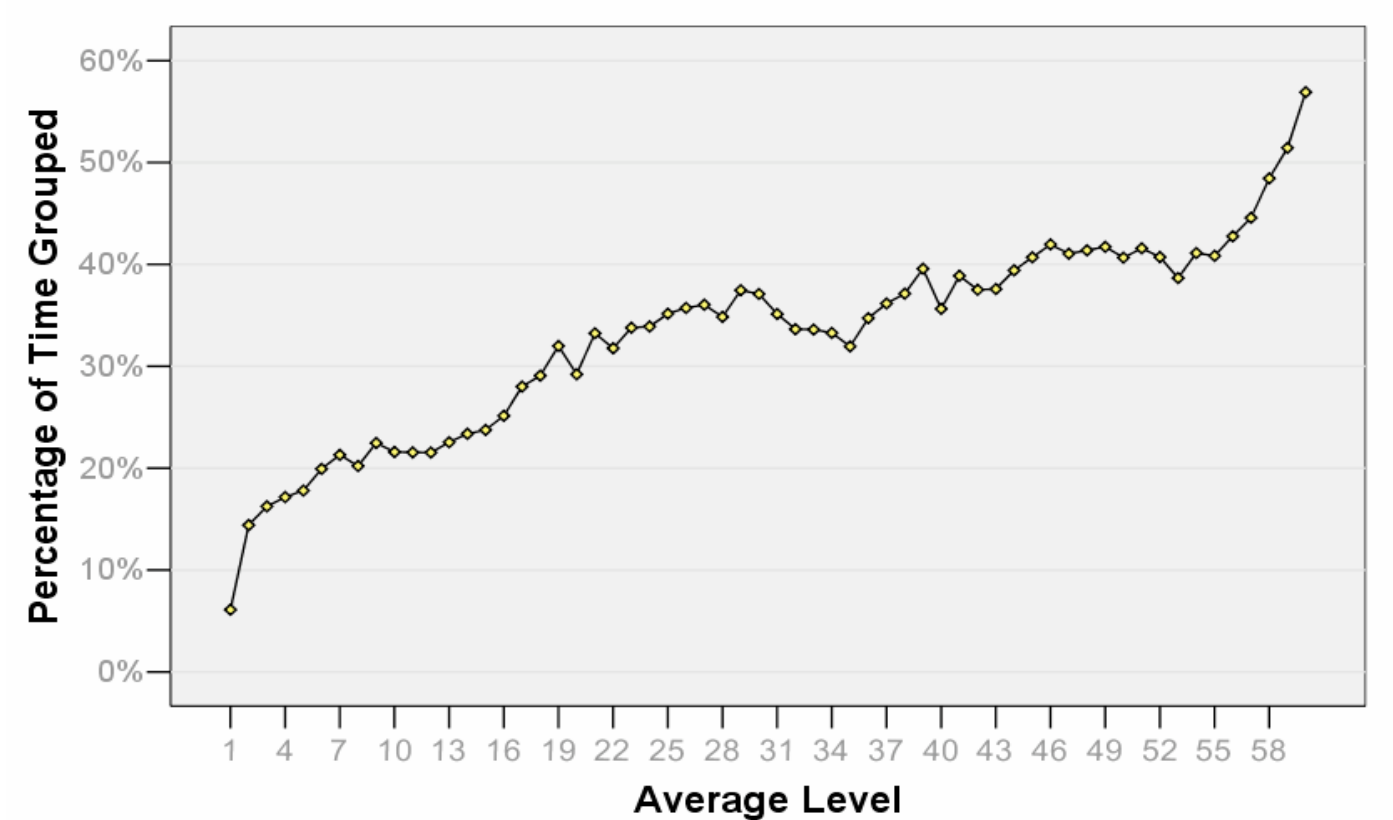
\includegraphics[scale=0.95]{./images/timespentgroup.png}
        \caption{Temps moyen passé en groupe, par classe}
        \label{timespentgroup}
        \end{figure}

\subsection{Jouer en guilde}
World Of Warcraft encourage les joueurs à former des groupes en utilisant deux mécanismes. Premièrement, pour qu'une complémentarité entre les habilitées des joueurs se crée. Deuxièmement, beaucoup de quêtes dans le jeux sont difficiles à réaliser tout seul. Nous pouvons aussi voir que des différences se dégagent entre le temps passé an groupe en fonction de chaque espèce (voir figure~\ref{tabltimegroup}.
\par Ces groupes sont appelés des guildes, elles sont un des aspects de la popularité de ce type de jeu. Dans World Of Warcraft, 66\% des avatars appartiennent à une guilde et que ce chiffre atteint 90\% si l'on tient compte que des joueurs ayant au moins le 43. Les joueurs appartenant à une guilde joue en moyenne plus souvent qu'un joueur sans guilde. 
	\begin{figure}[!h]
        \centering
        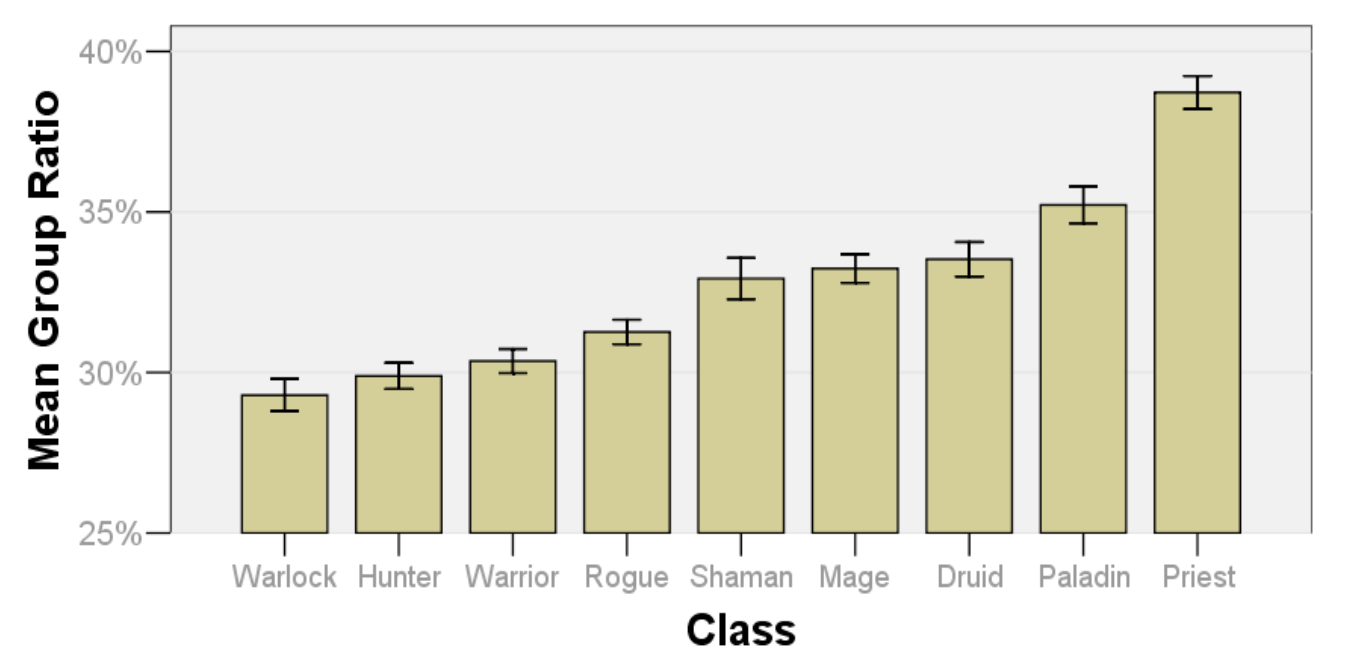
\includegraphics[scale=0.95]{./images/tabltimegroup.png}
        \caption{Temps moyen passé en groupe, par classe}
        \label{tabltimegroup}
        \end{figure}
\par Un des facteur important, pour essayer de réaliser un modèle de mobilité, est d'étudier la taille des guildes. La moyenne de personne dans une guilde est de 14,5\% (16,8\% si l'on exclut du calcul les guildes de une personne). Le median est de 6 (9 si l'on exclut du calcul les guildes de une personne). 

\subsection{Réseaux sociaux dans World Of Warcraft} 
Les auteurs ont mis en place un réseau social pour évaluer au mieux les guildes. Ils ont mis en place ce réseau selon deux méthodes différentes:
\begin{itemize}
	\renewcommand{\labelitemi}{$\bullet$}
	\item Une pour évaluer \textit{le potentiel de sociabilité des guildes:}\\
	Les joueurs sont connectés chacun aux autres (si en ligne au même moment),et cela sans tenir compte de leur localisation dans le jeu. Le réseau résultant reflète le spectre des opportunités des interactions sociales dans une guilde. Il va crée des liens entre les joueurs qui pourraient utiliser le "guild channel" et ceux qui font parti de la même guilde.
	\item Une pour quantifier \textit{les activités communes:}\\
	Les joueurs qui sont dans la même zone vont se connecter ensemble, sauf dans les grandes villes (Hotspots). Cette méthode permet de mettre en évidence les joueurs qui passent du temps ensemble, et qui se groupent en guilde pour exécuter des quêtes. Ces liens sont forts, car ils reflètent un intérêt mutuel. 
\end{itemize}

\par Les résultats montrent que les joueurs ne connaissent pas tous les joueurs du même guilde, et cela est d'autant plus vrai que le nombre de personne, dans la guilde, est important. Des sous groupes peuvent aussi apparaître dans les guildes, surtout pour les guildes avec un nombre de joueurs important. 
\par Dans la figure~\ref{co-location}, il est possible de voir à quoi ressemble les liens entre les différents joueurs d'une même guilde de 41 membres. Tout d'abord 17 membres de la guilde n'ont jamais été observé dans la même zone qu'un autre membre. Un noyau central se distingue, il est composé de 8 joueurs qui jouent souvent ensemble, 3 autres joueurs forment un trio central où les liens épais montrent qu'ils passent beaucoup de temps ensemble. Les autres joueurs jouent avec 2 (ou moins) membres de la guilde.
	 \begin{figure}[!h]
        \centering
        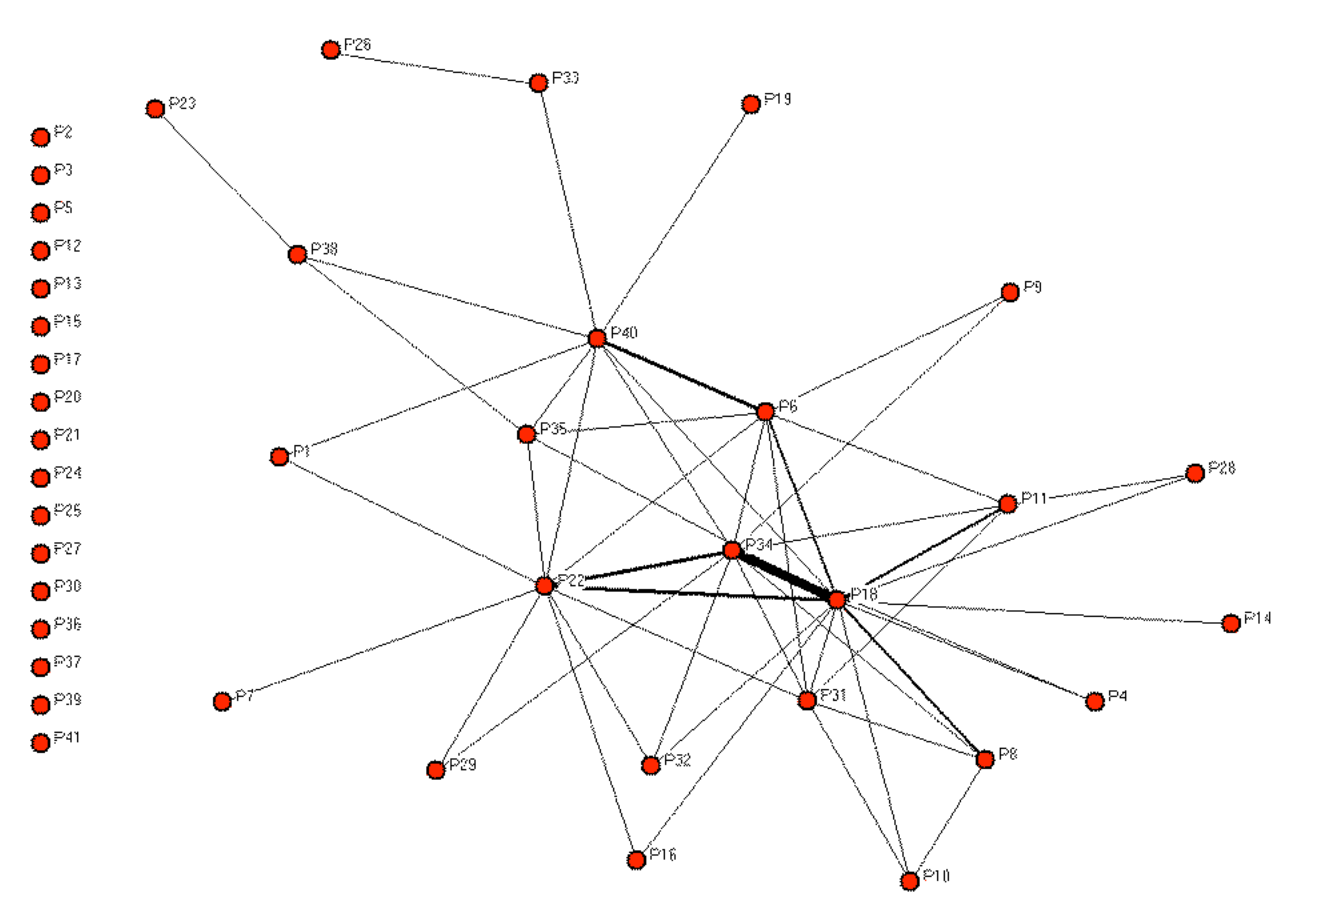
\includegraphics[scale=0.95]{./images/co-location.png}
        \caption{Co-location network dans une guilde de taille moyenne}
        \label{co-location}
        \end{figure}
\newpage
\section{Understanding Social Interaction in World of Warcraft}

Griffiths, Davies et Chappell~\cite{BreakingSteretype} ont trouvé que l'aspect favori de 41\% des joueurs, est les interactions sociales. De même Yee~\cite{1159988} a trouvé que 39,4\% des hommes et 53,3\% des femmes pensent que leurs amis, dans le jeu, sont comparables que leurs amis dans la "vie réelle". 
A FINIR (voir truc souligné) Quelques trucs intéressants mais aspect social par trop étude des mouvements.


\newpage
\bibliographystyle{plain}
\bibliography{Biblio}


 

\end{document}
